\section{处理器体系架构}

\subsection{Y86-64 指令集体系结构}

我们首先定义一个简单的指令集,作为我们处理器实现的运行示例。
因为受 x86-64 指令集的启发, 所以我们称我们的指令集为 Y86-64 指令集。
与 x86-64 相比, Y86-64 指令集的数据类型、指令和寻址方式都要少一些。
它的字节级编码也比较简单,机器代码没有相应的 x86-64 代码紧凑,不过设计它的 CPU 译码逻辑也要简单一些。
\begin{itemize}
    \item 寄存器: rax 、 rcx 、rdx 、 rbx 、rsp 、rbp 、rsi 、rdi 和 r8 到 r14 。
    \item 条件码: ZF(零标志)、SF(符号标志)、OF(溢出标志)
    \item 程序计数器:存放当前正在执行指令的地址。
    \item 状态码: AOK(正常)、 HLT(停止)、 ADR(地址错误)、 INS(无效指令)
    \item 内存:字节寻址的内存空间,小端法储存。
\end{itemize}

\subsubsection{Y86-64 指令}
\paragraph{指令编码}
\begin{figure}[H]
    \centering
    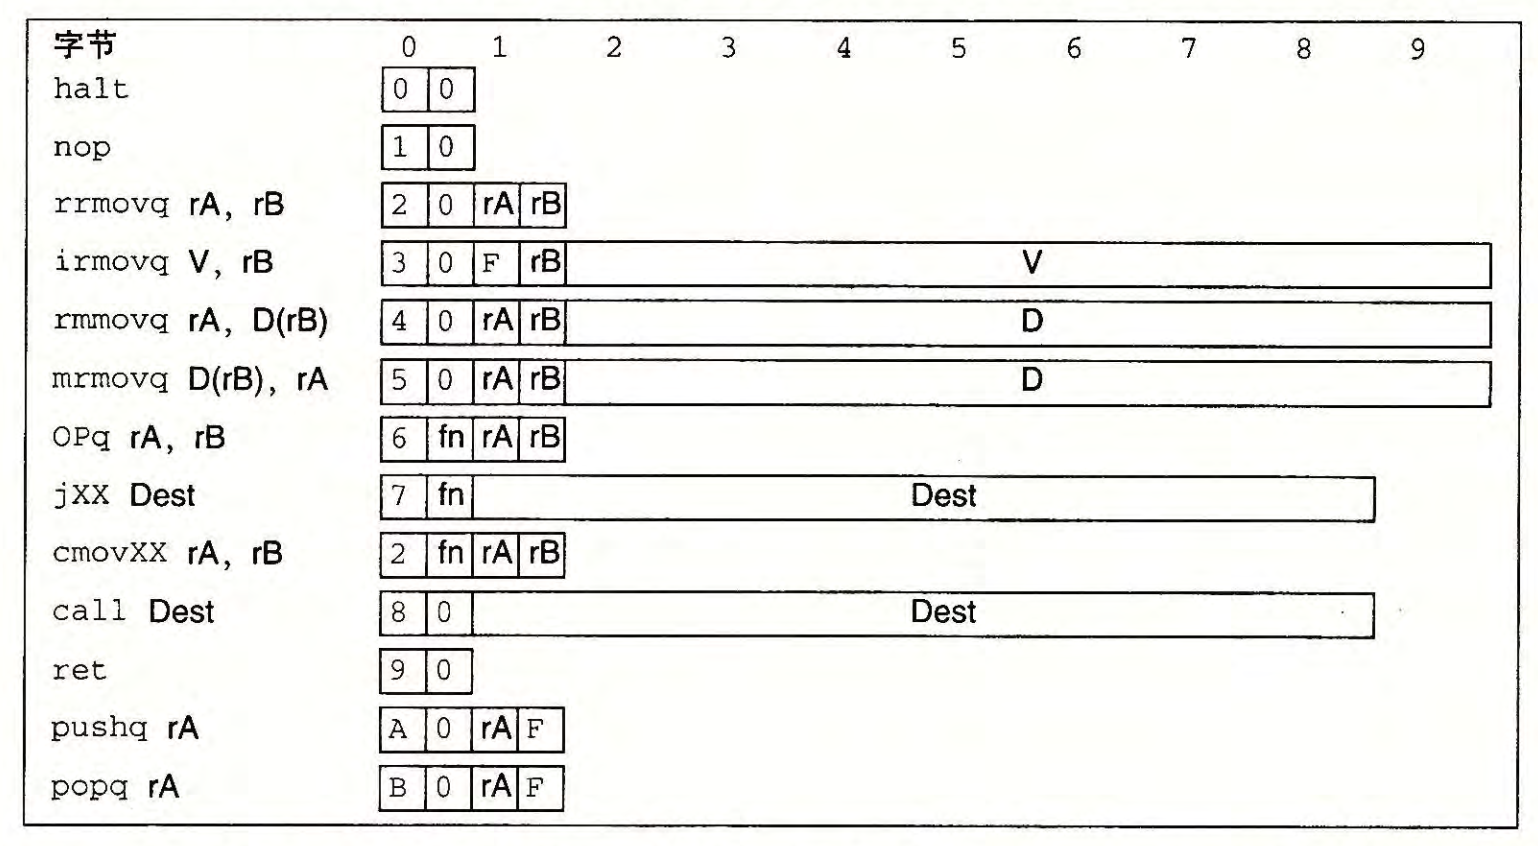
\includegraphics[width=0.8\textwidth]{instruction-encode.png}
\end{figure}
\begin{figure}[H]
    \centering
    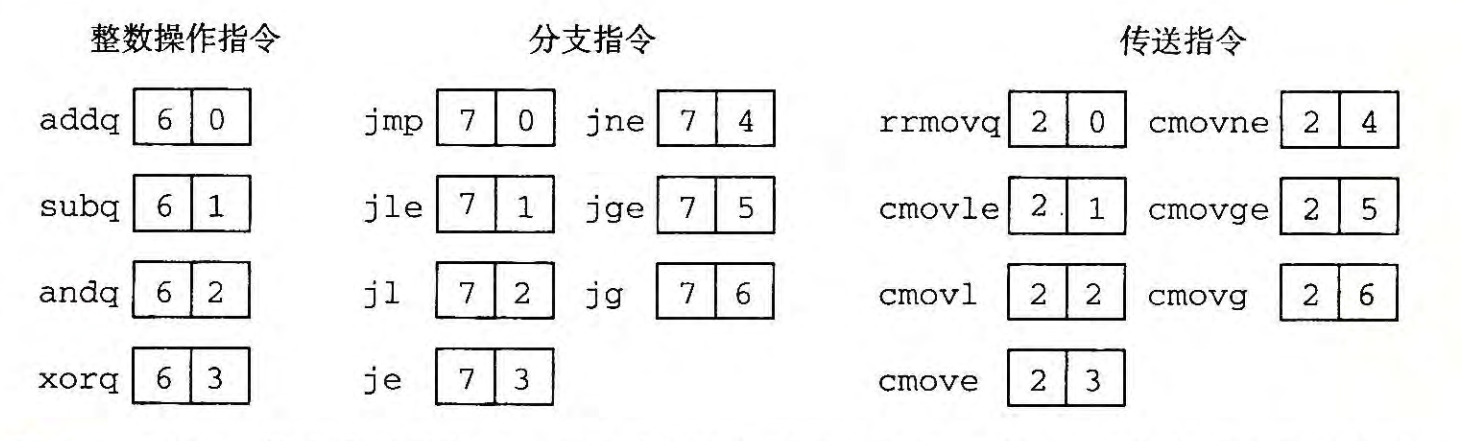
\includegraphics[width=0.8\textwidth]{instruction-function-encode.png}
\end{figure}

\begin{itemize}
    \item x86-64 的 movq 指令分成了 4 个不同的指令: irmovq 、 rrmovq 、 mrmovq 和 rmmovq 。分别显式地指明源和目的的格式。
    \item 内存引用方式是简单的基址和偏移量形式。在地址计算中,不支持第二变址寄存器 (second index register) 和任何寄存器值的伸缩 (scaling)。
    \item 4 个整数操作指令 (OPq) : addq 、 subq 、 andq 和 xorq 。 它们只对寄存器数据进行操作,会设置 3 个条件码 ZF 、 SF 和 OF 。
    \item 7 个跳转指令 (jXX) : jmp 、 jle 、 jl 、 je 、 jne 、 jge 和 jg 。 它们根据条件码的值来决定是否跳转。
    \item 有 6 个条件传送指令 (cmovXX) : cmovle 、 cmovl 、 cmove 、 cmovne 、 cmovge 和 cmovg 。 它们根据条件码的值来决定是否执行传送操作。
    \item call 指令将返回地址入栈,然后跳到目的地址。 ret 指令从这样的调用中返回。
    \item pushq 和 popq 指令实现了入栈和出栈操作。
    \item halt 指令停止指令的执行。
    \item nop 指令什么也不做,只是简单地前进到下一条指令。
\end{itemize}

每条指令需要 1~10 个字节不等,这取决于需要哪些字段。每条指令的第一个字节表明指令的类型。这个字节分为两个部分,每部分 4 位:高 4 位是代码 (code) 部分,低 4 位是功能 (function) 部分。

\paragraph{寄存器编码}
\begin{figure}[H]
    \centering
    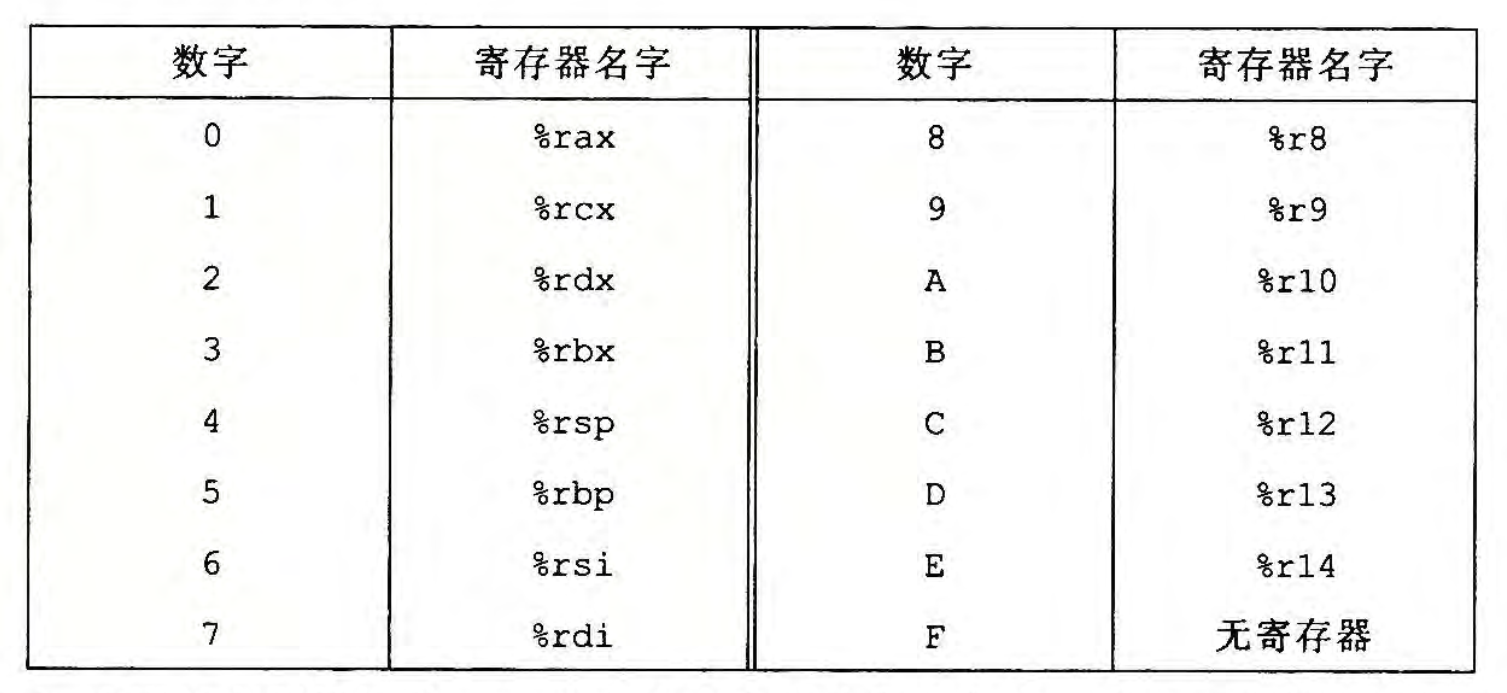
\includegraphics[width=0.8\textwidth]{register-encode.png}
\end{figure}

15 个程序寄存器中每个都有一个相对应的范围在 0 到 OxE 之间的寄存器标识符 (register ID) 。 当需要指明不应访问任何寄存器时,就用 ID 值 OxF 来表示。

\subsubsection{Y86-64 异常}

\begin{figure}[H]
    \centering
    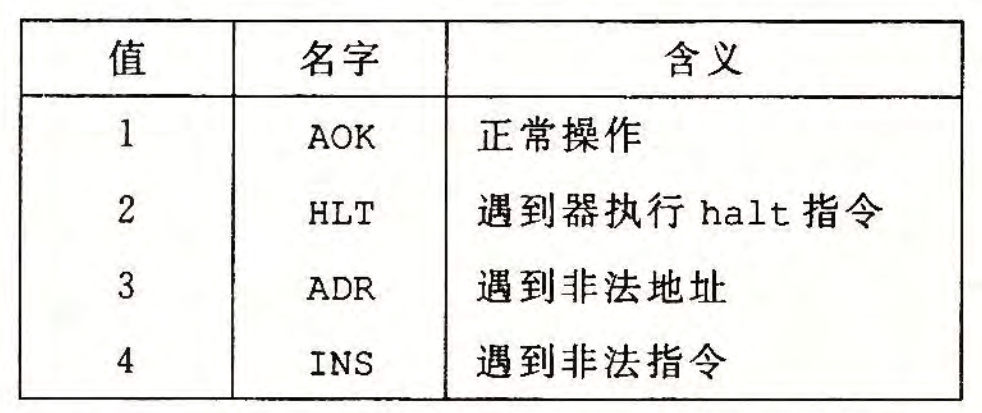
\includegraphics[width=0.6\textwidth]{status-code.png}
\end{figure}

Y86-64 中的状态码描述程序执行的总体状态。正常执行时,状态码为 AOK 。当程序执行 halt 指令时,状态码变为 HLT 。如果程序试图访问无效的内存地址,状态码变为 ADR 。如果程序试图执行无效指令,状态码变为 INS 。
对于 Y86-64, 当遇到这些异常的时候,我们就简单地让处理器停止执行指令。在更完整的设计中,处理器通常会调用一个异常处理程序(exception handler), 这个过程被指定用来处理遇到的某种类型的异常。

\subsubsection{Y86-64 程序}
\begin{lstlisting}[style=ASMStyle]
; Execution begins at address 0
        .pos 0
        irmovq stack, %rsp      ; Set up stack pointer
        call main               ; Execute main program
        halt                    ; Terminate program

; Array of 4 elements
array:  .align 8
        .quad 0x000d000d000d
        .quad 0x00c000c000c0
        .quad 0x0b000b000b00
        .quad 0xa000a000a000

main:
        irmovq array, %rdi
        irmovq $4, %rsi
        call sum                ; sum(array, 4)
        ret

; long sum(long *start, long count)
; start in %rdi, count in %rsi
sum:
        irmovq $8, %r8          ; Constant 8
        irmovq $1, %r9          ; Constant 1
        xorq %rax, %rax         ; sum = 0
        andq %rsi, %rsi         ; Set CC
        jmp     test            ; Goto test
loop:
        mrmovq (%rdi), %r10     ; Get *start
        addq %r10, %rax         ; Add to sum
        addq %r8, %rdi          ; start++
test:
        subq %r9, %rsi          ; count--. Set CC
        jne     loop            ; Stop when 0
        ret                     ; Return

; Stack starts here and grows to lower addresses
        .pos 0x200
stack:
\end{lstlisting}

注意到:
\begin{itemize}
    \item 由于 Y86-64 是一个简化的指令集,所以相较于 x86-64, Y86-64 的汇编代码会更加复杂。
    \item 程序从地址 0 处开始。
    \item 初始化栈指针,指明地址 0x200 处是栈的起始位置,低地址增长。须保证栈不会增长得太大以至千覆盖了代码或者其他程序数据。
\end{itemize}

\begin{sidenote}{两个特别的指令}
    在 Y86-64 和 x86-64 中:
    \begin{itemize}
        \item pushq \%rsp 会压入 \%rsp 的原始值。
        \item popq \%rsp 会将 \%rsp 置为从内存中读出的值。
    \end{itemize}
\end{sidenote}

\subsection{逻辑设计}